%Segunda Unidad
\section{Aproximación de funciones}
%==========================================================================
\begin{frame}{Teorema de aproximación de polinomios}
\begin{Teo}[Weierestrass]
Suponga que $f$ está definida y es continua en $[a, b]$. Para cada $\epsilon>0$, existe un polinomio $P(x)$, con la propiedad de que 
$$|f(x)-P(x)|<\epsilon, \quad \forall x \in [a, b]$$
\end{Teo}
\indent Los polinomios son ampliamente utilizados para la interpolación numérica porque:
\begin{itemize}
\item Aproximan de manera uniforme a las funciones conitnuas. 
\item Tienen derivadas e integrales fáciles de calcular. Además, sus integrales y derivadas también son polinomios. 
\end{itemize}
\indent Las principales limitaciones de los polinomios de Taylor son:
\begin{itemize}
\item Generalmente no ofrecen una buena aproximación en todo un intervalo, sino que la aproximación se concentra alrededor de $x_0$.
\item Aumentar el grado del polinomio de Taylor no necesariamente brindará una mejor aproximación.   
\item No utilizan más que un único punto para definir el polonomio.  
\end{itemize}
\end{frame}
%===========================================================================
\begin{frame}{Limitaciones de los polinomios de Taylor}
\indent Debido a las limitaciones expuestas, los polinomios de Taylor se usan principalmente para:
\begin{enumerate}
\item Derivación de otros métodos numéricos, como el método de diferencias finitas.
\item Estimación del error
\end{enumerate}
\label{TeoremaTaylor}
\begin{Teo}[Teorema de Taylor]
Suponga que $f\in C^n[a,b]$, $f^{(n+1)}$ esta definida en $[a,b]$ y $x_0\in[a,b]$. Entonces, para cada $x\in[a,b]$, existe $\xi(x)\in (x_0,x)$ (si $x>x_0$ y $\xi(x)\in(x,x_0)$ en el otro caso)  tal que: 
\begin{itemize}
\item $f(x)=P_n(x)+R_n(x)$ donde
\item $P_n(x)=\displaystyle \sum_{k=0}^{n}\dfrac{f^{(k)}(x_0)}{k!}(x-x_0)^k$ y
\item $R_n(x)=\dfrac{f^{(n+1)}(\xi(x))}{(n+1)!}(x-x_0)^{(n+1)}$.
\end{itemize}
\hyperlink{DeduccionFormulaSegundoOrden}{\textcolor{cyan}{Regreso a fórmula de segundo orden.}}
\end{Teo}
\end{frame}
%==========================================================================
\label{RetornoPolinomioLagrange}
\begin{frame}{Polinomio interpolante de Lagrange I}
\begin{Teo}[Polinomios de Lagrange]
\indent Si $f$ es una funcion definida en los diferentes valores $\{x_0,\cdots, x_n\}$, entonces existe un único polinomio $P(x)$ de grado a lo más $n$, con la propiedad:
$$f(x_k)=P(x_k)\quad k=0, 1, \dots, n$$
El polinomio $P(x)$ se define como sigue:
\begin{align*}
P(x)&=\sum_{k=0}^{n}f(x_k)L_{n,k}(x)=f(x_0)L_{n,0}+\cdots+f(x_n)L_{n,n}
\end{align*}
donde
$$L_{n,k}=\frac{(x-x_0)(x-x_1)\dots(x-x_{k+1})(x-x_{k+1})\dots (x-x_n)}{(x_k-x_0)(x_k-x_1)\dots(x_k-x_{k+1})(x_k-x_{k+1})\dots (x_k-x_n)}$$
\end{Teo}
\end{frame}
%==========================================================================
\begin{frame}{Polinomio interpolante de Lagrange II}
\begin{Teo}[Error del polinomio de Lagrange]
Suponga que $x_0, x_1, \dots, x_n$ son números distintintos en el intervalo $[a,b]$ y que $f \in C^{n+1}[a,b]$. Entonces, para cada x en $[a,b]$ existe in número $\xi(x)$ en $(a,b)$ con 
$$f(x)=P(x)+\frac{f^{(n+1)}(\xi(x))}{(n+1)!}(x-x_0)(x-x_1)\dots (x-x_n)$$
donde $P(x)$ es el polinomio interpolante de Lagrange.
\end{Teo}
\hyperlink{PolinomioLagrange}{\textcolor{cyan}{Enlace a ejercicio.}}
\end{frame}
%==========================================================================
\begin{frame}{Interpolación, Spline Cúbicos I}
\indent Considere el siguiente ajuste polinomial:
\begin{multicols}{2}
\begin{figure}[H]
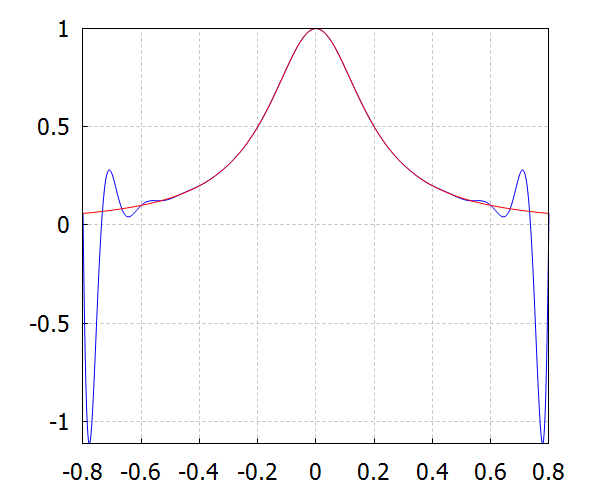
\includegraphics[scale=0.6]{Imagen21}
\caption{\scriptsize En la figura se observa la interpolación por polinomios de Lagrange para $f(x)=\dfrac{1}{1+25x^2}$ para $x\in[-1,1]$ con 30 puntos equidistante comenzando en -1 y finalizando en 1.}
\end{figure}
En este ejemplo se demuestra que los polinomios de alto orden (en el ejemplo de la figura tendríamos un polinomio de orden 31)  pueden oscilar erráticamente. Evidentemente esta característica es indeseable en muchas situaciones; en este apartado se mostrará una técnica que puede evitar este problema siempre con la idea de hacer un ajuste polinomial.
\end{multicols}
\end{frame}
%==========================================================================
\begin{frame}{Interpolación, Spline Cúbicos II}
\indent Los ingredientes para construir un \textbf{spline} (esta palabra no tiene traducción al español, su significado es "larga tira flexible") \textbf{cúbico interpolante} $S$ de alguna función $f$ se basan en las siguiente consideraciones:
\begin{itemize}
\item Una función $f$ de variable real definida en el intervalo $[a,b]$.
\item Una partición del intervalo $[a,b]$; $a=x_0<x_1<\cdots<x_n=b$.
\item $S(x)$ restringido a $[x_j,x_{j+1}]$ es un polinomio cúbico para cada $j=0,\cdots, n-1$. A esta parte se le denota por $S_j(x)$.
\item $S_j(x_j)=f(x_j)$ y $S_{j}(x_{j+1})=f(x_{j+1})$ para cada $j=0,\cdots, n-1$.
\item $S'_{j+1}(x_{j+1})=S'_{j}(x_{j+1})$ para cada $j=0,\cdots, n-2$.
\item $S''_{j+1}(x_{j+1})=S''_{j}(x_{j+1})$ para cada $j=0,\cdots, n-2$.
\item Si $S''(x_0)=S''(x_n)=0$ se dice que es un \textbf{Spline de frontera natural}. Si $S'(x_0)=f'(x_0)$ y $S'(x_n)=f'(x_n)$ se dice que es un \textbf{Spline con frontera sujeta}. 
\end{itemize}
\end{frame}
%==========================================================================
\begin{frame}{Interpolación, Spline Cúbicos III}
\begin{figure}
\begin{center}
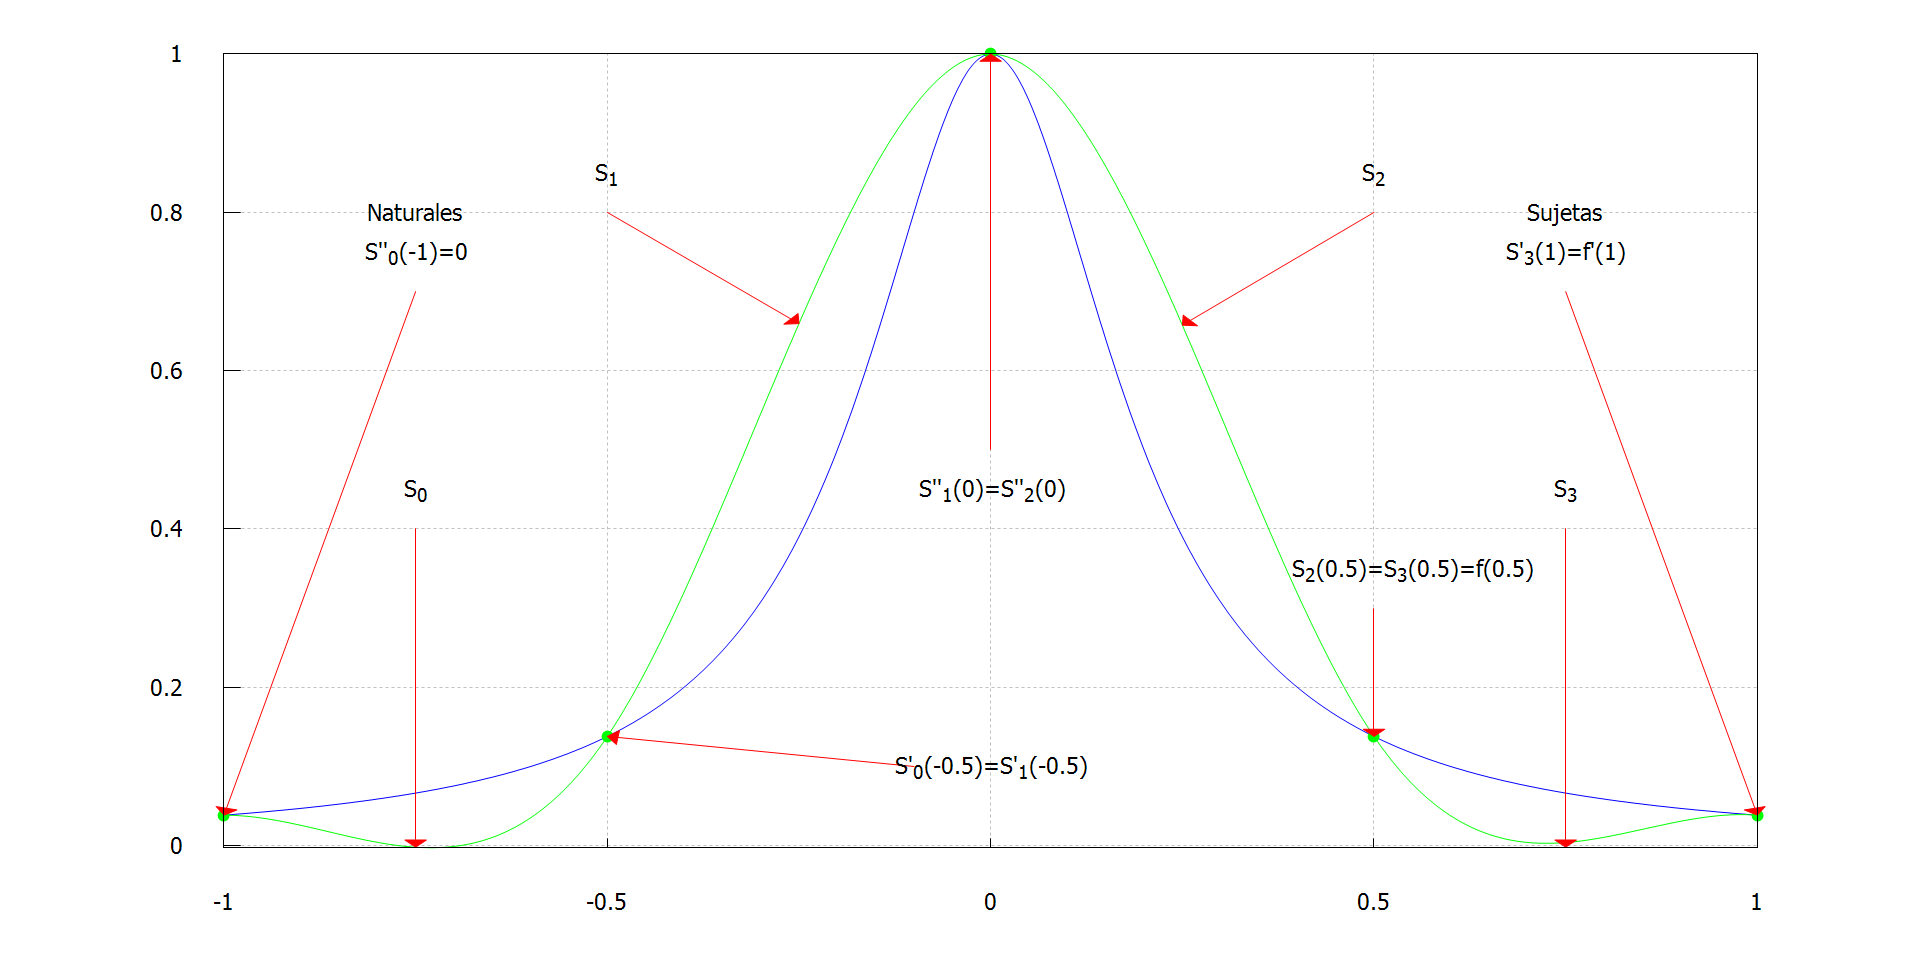
\includegraphics[scale=0.4]{Imagen22}
\end{center}
\caption{Aquí se muestran algunas condiciones de los spline. La función que se ve arriba en azul es $f(x)=\dfrac{1}{1+25x^2}$. En verde se observan los splines cúbicos.}
\end{figure}
\end{frame}
%==========================================================================
\begin{frame}{Interpolación, Spline Cúbicos IV}
\begin{Def}[Fórmulas de recurrencia para los Splines Cúbicos]
\small
\indent Definanse los Splines Cúbicos de la función $f$ definida en $[x_0,x_n]$:
\begin{center}
$S(x)=S_j(x)\equiv a_j+b_j(x-x_j)+c_j(x-x_j)^2+d_j(x-x_j)^3$\\ para $x\in[x_j,x_{j+1}]$ donde $j=0,\cdots, n-1$.
\end{center}
\indent Por comodidad definanse los siguientes elementos:
\begin{center}
$a_n\equiv f(x_n)$, $b_n\equiv S'(x_n)$, $c_n\equiv S''(x_n)/2$, $h_j\equiv x_{j+1}-x_j$, $j=0,\cdots, n-1$.
\end{center}
\indent Las siguientes ecuaciones de recurrencia deben ser verificadas para que los $S_j$ cumplan con las condiciones de un Spline Cúbico.
\begin{enumerate}
\item $a_j\equiv f(x_j)$ para $j=0,\cdots, n-1$.
\item $a_j+b_jh_j+c_jh_j^2+d_jh_j^3=a_{j+1}$ para $j=0,\cdots, n-1$.
\item $b_j+2c_jh_j+3d_jh_j^2=b_{j+1}$ para $j=0,\cdots, n-1$.
\item $c_j+3d_jh_j=c_{j+1}$ para $j=0,\cdots, n-1$.
\item $\dfrac{3}{h_j}(a_{j+1}-a_j)-\dfrac{3}{h_{j-1}}(a_j-a_{j-1})=h_{j-1}c_{j-1}+2(h_{j-1}+h_j)c_j+h_jc_{j+1}$ para $j=1,\cdots, n-1$.
\end{enumerate}
\end{Def}
\end{frame}
%==========================================================================
\begin{frame}{Interpolación, Spline Cúbicos V}
\indent Las ecuaciones en el numeral 5 permiten resolver para los $\{c_j\}$; luego en el numeral 4 se pueden resolver los $\{d_j\}$ y con el numeral 2 se pueden encontrar los $\{b_j\}$. Los $\{a_j\}$ son conocidos desde el principio y con ello se pueden encontrar los Splines Cúbicos. \\
\indent Si se recuerda, $c_j$ está definido para $j=0,\cdots n$. Entonces es necesario encontrar $n+1$ valores. La ecuación en el numeral 5 solo provee de $n-1$ ecuaciones; por lo tanto faltan dos ecuaciones más que se podrán obtener de considerar las condiciones en la frontera (naturales o fijas). 
\end{frame}
%==========================================================================
\begin{frame}{Mínimos cuadrados I}
Considere el siguiente conjunto de datos $\{(x_i,y_i)\}_{i=1}^{N}$ asociados:
\begin{displaymath}
\begin{bmatrix}
1&2&3&4&5&6&7&8&9&10\\
\downarrow &\downarrow &\downarrow &\downarrow &\downarrow &\downarrow &\downarrow &\downarrow &\downarrow &\downarrow\\
3&5&9&11&15&17&20&24&26&29
\end{bmatrix}
\end{displaymath}
Abajo se aprecian los pares ordenados correspondientes a cada par asociado:
\begin{figure}[H]
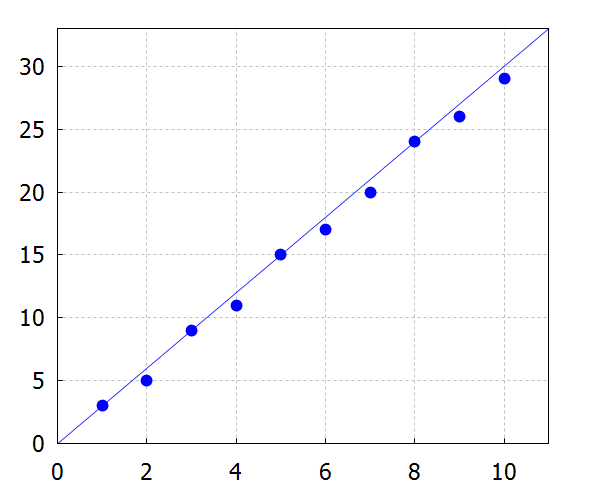
\includegraphics[scale=0.55]{Imagen2}
\caption{Recta de aproximación a los pares ordenados.}
\end{figure}
\end{frame}
%==========================================================================
\begin{frame}{Mínimos cuadrados II}
\indent El objetivo consiste en determinar la recta $Y=a_1X+a_0$ que mejor modele al conjunto de datos asociados.\\
\indent Existen algunos enfoques para encontrar esta recta:
\begin{Def}[Problema Minimax]
\centering $\displaystyle \min_{a_0,a_1}\max_{1\leq i\leq 10}|y_i-(a_1x_i-a_0)|$
\end{Def}
\begin{Def}[Problema de desviación absoluta]
\centering $\displaystyle \min_{a_0,a_1}\sum_{i=1}^{10}|y_i-(a_1x_i-a_0)|$
\end{Def}
\begin{Def}[Problema de mínimos cuadrados]
\centering $\displaystyle \min_{a_0,a_1}\sum_{i=1}^{10}|y_i-(a_1x_i-a_0)|^2=\displaystyle \min_{a_0,a_1}\sum_{i=1}^{10}(y_i-(a_1x_i-a_0))^2$
\end{Def}
\end{frame}
%==========================================================================
\begin{frame}{Mínimos cuadrados III}
\indent A continuación se mostrará una forma muy conocida para la deducción del método de mínimos cuadrados; para ello defina los siguientes vectores:
\begin{align*}
X=&[x_1,\cdots,x_n]^T\\
Y=&[y_1,\cdots,y_n]^T\\
U=&[1,\cdots,1]^T
\end{align*}
\indent Entonces podemos pensar en el problema de ajuste de la siguiente manera: Deseamos encontrar $a_0$ y $a_1$ tales que
$$a_1X+a_0U=Y$$
De forma matricial esto sería:
\begin{displaymath}
(X|U)
\left(
\begin{array}{c}
a_1\\
a_0
\end{array}
\right)=Y
\end{displaymath}
\end{frame}
%==========================================================================
\begin{frame}{Mínimos cuadrados IV}
\indent Si ahora se multiplica por la transpuesta de la primer matriz, se obtine:
\begin{displaymath}
\left(
\begin{array}{c}
X^T\\
U^T
\end{array}
\right)
(X|U)
\left(
\begin{array}{c}
a_1\\
a_0
\end{array}
\right)=
\left(
\begin{array}{c}
X^T\\
U^T
\end{array}
\right)
Y
\end{displaymath}
\indent Esto es equivalente a lo siguiente:
\begin{displaymath}
\left(
\begin{array}{cc}
X^TX &X^TU\\
U^TX & U^TU
\end{array}
\right)
\left(
\begin{array}{c}
a_1\\
a_0
\end{array}
\right)=
\left(
\begin{array}{c}
X^TY\\
U^TY
\end{array}
\right)
\end{displaymath}
\indent Como se puede apreciar, resolviendo este sistema podemos encontrar las soluciones para los coeficientes de la regresión lineal. \\
\indent Ahora considere le problema siguiente: Se desan encontrar los valores $[a_m,a_{m-1},\cdots,a_0]$ de manera tal que:
$$a_mX^m+\cdots+a_1X+a_0U=Y,$$
\indent donde $X^k=[x_1^k,\cdots,x_n^k]^T$. Nuevamente esto se puede escribir como el siguiente sistema:
\end{frame}
%==========================================================================
\begin{frame}{Mínimos cuadrados V}
\textcolor{red}{
\begin{displaymath}
(X^m|X^{m-1}|\cdots X|U)
\left(
\begin{array}{c}
a_m\\
\vdots\\
a_0
\end{array}
\right)=Y
\end{displaymath}
}
\indent Multiplicando por la transpuesta:
\begin{displaymath}
\left(
\begin{array}{c}
(X^m)^T\\
\vdots\\
(X)^T\\
U^T
\end{array}
\right)
(X^m|X^{m-1}|\cdots X|U)
\left(
\begin{array}{c}
a_m\\
\vdots\\
a_0
\end{array}
\right)=
\left(
\begin{array}{c}
(X^m)^T\\
\vdots\\
(X)^T\\
U^T
\end{array}
\right)
Y
\end{displaymath}
Lo que termina siendo equivalente a resolver el sistema:
\begin{displaymath}
\left(
\begin{array}{cccc}
(X^m)^TX^m & (X^m)^TX^{m-1} &\hdots & (X^m)^TU\\
\vdots&\vdots &&\vdots\\
(X)^TX^m&(X)^TX^{m-1}&\hdots &(X)^TU\\
U^TX^m&U^TX^{m-1}&\hdots &U^TU
\end{array}
\right)
\left(
\begin{array}{c}
a_m\\
\vdots\\
a_0
\end{array}
\right)=
\left(
\begin{array}{c}
(X^m)^TY\\
\vdots\\
(X)^TY\\
U^TY
\end{array}
\right)
\end{displaymath}
\end{frame}
%==========================================================================
\begin{frame}{Derivación Numérica I}
\small
\label{DeduccionFormulaSegundoOrden}
\hyperlink{TeoremaTaylor}{\textcolor{cyan}{Enlace al teorema de Taylor.}}
\indent Aquí se mostrará una manera estándar de deducir la fórmula numérica para la aproximación de la segunda derivada por medio de la fórmula de Taylor:
\begin{displaymath}
\scriptsize
\begin{array}{rl}
\renewcommand{\arraystretch}{1.5}
f(x+h)= &\textcolor{red}{f(x)+f'(x)h+\dfrac{f''(x)}{2}h^2+\dfrac{f^{(3)}(x)}{6}h^3+\dfrac{f^{(4)}(\xi)}{24}h^4}.\\\pause
f(x-h)=&\textcolor{red}{f(x)+f'(x)(-h)+\dfrac{f''(x)}{2}(-h)^2+\dfrac{f^{(3)}(x)}{6}(-h)^3+\dfrac{f^{(4)}(\eta)}{24}(-h)^4}\\\pause
=&\textcolor{red}{f(x)-f'(x)h+\dfrac{f''(x)}{2}h^2-\dfrac{f^{(3)}(x)}{6}h^3+\dfrac{f^{(4)}(\eta)}{24}h^4}\\\pause
&\rule{7cm}{0.01cm}\\
f(x+h)+f(x-h)=&\textcolor{cyan}{2f(x)+f''(x)h^2+\dfrac{f^{(4)}(\eta)}{24}h^4+\dfrac{f^{(4)}(\xi)}{24}h^4}\\\pause
=&\textcolor{cyan}{2f(x)+f''(x)h^2+\dfrac{f^{(4)}(\eta)+f^{(4)}(\xi)}{2}\dfrac{1}{12}h^4}\\\pause
=&\textcolor{cyan}{2f(x)+f''(x)h^2+f^{(4)}(\theta)\dfrac{1}{12}h^4}\\
\end{array}
\end{displaymath}
Despejando finalmente para $f''(x)$ se obtiene una aproximación a la segunda deriva:
\begin{Def}[Aproximación de la segunda derivada]
$$f''(x)\approx\dfrac{f(x+h)-2f(x)+f(x-h)}{h^2}$$
\end{Def}
\end{frame}
%=========================================================================
\begin{frame}{Integración Numérica I}
\indent Suponga que se quiere encontrar el valor de la siguiente integral usando los métodos vistos en cálculo (integración por partes, cambio de variables,...etc):
$$\int_{0}^{a}\sqrt{1+\cos^2(x)}dx$$
\indent Si se intentara hacer, nos daríamos cuenta de que es un problema bastante complicado; de hecho se puede demostrar formalmente que el problema es irresoluble planteado en estos términos. 
\begin{Def}[Técnica de cuadratura]
La \textit{técnica de cuadratura}  consiste en encontrar unos valores (denominados pesos) $\{a_0,\cdots,a_n\}$ correspondientes a los puntos $\{x_0,\cdots, x_n\}$ en el intervalo $[a,b]$  de manera que: 
$$\int_{a}^{b}f(x)dx\approx \sum_{k=0}^{n}a_kf(x_k)$$
\end{Def}
\end{frame}
%=========================================================================
\begin{frame}{Integración Numérica II}
\begin{figure}[H]
\centering
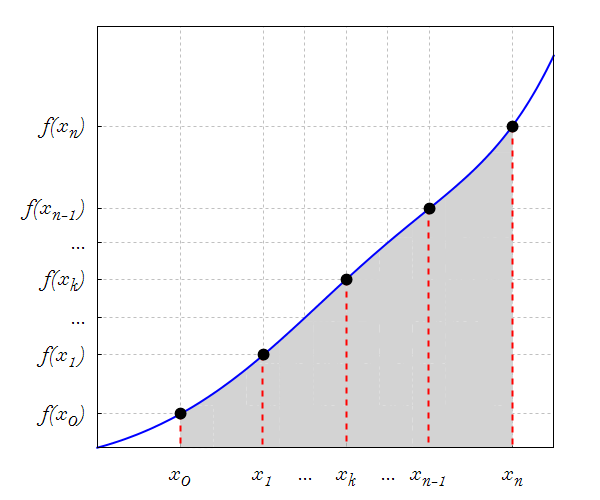
\includegraphics[scale=0.6]{Imagen62}
\end{figure}
\begin{displaymath}
\begin{array}{rl}
\int_a^b f(x)dx=&\textcolor{red}{\int_a^b\sum_{k=0}^n f(x_k)L_k(x)dx+\int_a^b\prod_{k=0}^{n}(x-x_k)\dfrac{f^{(n+1)}(\xi(x))}{(n+1)!}}\\
=&\textcolor{cyan}{\sum_{k=0}^n f(x_k)\int_a^b L_k(x)dx+\int_a^b\prod_{k=0}^{n}(x-x_k)\dfrac{f^{(n+1)}(\xi(x))}{(n+1)!}}
\end{array}
\end{displaymath}
\end{frame}
%=========================================================================
\begin{frame}{Integración Numérica III}
\indent Comparando con la ténica de cuadratura, se observa que se pueden escoger los $a_k$ de manera tal que: 
$$\textcolor{red}{a_k=\int_a^b L_k(x)dx}$$\\
El error como se puede ver es igual a:
$$\textcolor{cyan}{E(f)=\int_a^b\prod_{k=0}^{n}(x-x_k)\dfrac{f^{(n+1)}(\xi(x))}{(n+1)!}}$$
\begin{Teo}[Valor medio para integrales]
Suponga que $f\in C[a,b]$, $g$ es Riemann integrable en $[a,b]$ y que $g$ no cambia de signo en $[a,b]$. Entonces existe un número $c\in (a,b)$ tal que:
$$\int_{a}^{b}f(x)g(x)dx=f(c)\int_a^bg(x)dx.$$
\end{Teo}
\end{frame}
%=========================================================================
\begin{frame}{Integración Numérica IV}
\label{CuadraturaTeoremaValorMedio}
\hyperlink{EjercicioCuadraturaError}{\textcolor{cyan}{Ejercicio de estimación del error.}}
\begin{Def}[Regla del trapecio]
\centering $\displaystyle \int_a^b f(x)dx\approx \dfrac{b-a}{2}[f(a)+f(b)]$
\end{Def}
\begin{figure}[H]
\centering
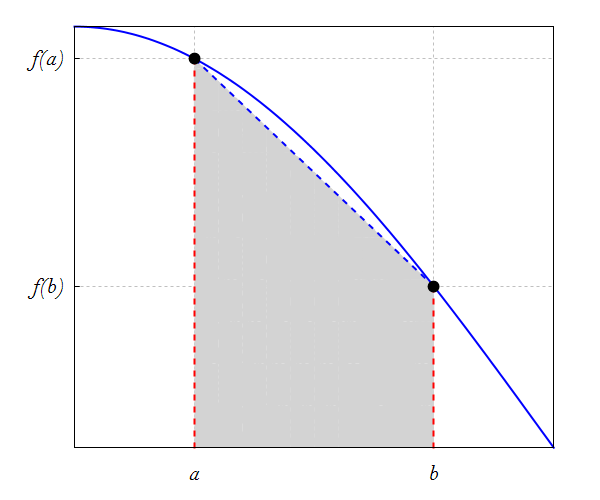
\includegraphics[scale=0.6]{Imagen24}
\caption{Como se puede apreciar en la figura, el nombre de la regla proviene de la fórmula del área de un trapecio de altura $b-a$ y bases $f(a)$, $f(b)$.}
\end{figure}
\end{frame}
%=========================================================================
\begin{frame}{Integración Numérica V}
\small
\vspace*{-0.5cm}
\indent Se deducirá la regla de Simpson, donde $x_0,x_1$ y $x_2$ son puntos equidistantes en $[a,b]$ con $x_0=a$ y $x_2=b$.
\begin{displaymath}
\begin{array}{rl}
\displaystyle \int_{x_0}^{x_2} f(x)dx=&\bigg[f(x_1)x+\dfrac{f'(x_1)}{2}(x-x_1)^2+\dfrac{f''(x_1)}{6}(x-x_1)^3\\
&+\dfrac{f^{(3)}(x_1)}{24}(x-x_1)^4\bigg]_{x_0}^{x_2}+\dfrac{1}{24}\displaystyle \int_{x_0}^{x_2}f^{(4)}(\xi(x))(x-x_1)^4dx\\
=&\bigg[f(x_1)x+\dfrac{f'(x_1)}{2}(x-x_1)^2+\dfrac{f''(x_1)}{6}(x-x_1)^3\\
&+\dfrac{f^{(3)}(x_1)}{24}(x-x_1)^4\bigg]_{x_0}^{x_2}+\displaystyle f^{(4)}(\xi)\dfrac{1}{24}\int_{x_0}^{x_2}(x-x_1)^4dx\\
=&2hf(x_1)+\dfrac{h^3}{3}f''(x_1)+\dfrac{f^{(4)}(\xi)}{60}h^5\\
=&2hf(x_1)+\dfrac{h^3}{3}(\textcolor{red}{\dfrac{1}{h^2}[f(x_0)-2f(x_1)+f(x_2)]-\dfrac{h^{2}}{12}f^{(4)}(\theta)})\\
&+\dfrac{f^{(4)}(\xi)}{60}h^5\approx \dfrac{h}{3}[f(x_0)+4f(x_1)+f(x_2)]
\end{array}
\end{displaymath}
\end{frame}
%=========================================================================
\begin{frame}{Integración Numérica VI}
\begin{Def}[Regla de Simpson]
\centering $\displaystyle \int_{x_0}^{x_2} f(x)dx\approx \dfrac{h}{3}[f(x_0)+4f(x_1)+f(x_2)]$
\end{Def}
\small
\begin{Def}[Grado de Precisión]
Se dice que una fórmula de cuadratura tiene \textbf{grado de precisión $n$} si $n$ es el entero positivo más grande tal que esta fórmula es exacta para $x^k$ para $k=0,1,\cdots, n$.  
\end{Def}
¿Cuál es el grado de precisión de la regla de Simpson? Se puede verificar que:
\begin{displaymath}
\textcolor{red}{
\begin{array}{rll}
\int_{x-h}^{x+h}s^0ds=&\dfrac{h}{3}((x-h)^0+4x^0+(x+h)^0)=2h\\\pause
\int_{x-h}^{x+h}sds=&\dfrac{h}{3}((x-h)+4x+(x+h))=2hx\\\pause
\int_{x-h}^{x+h}s^2ds=&\dfrac{h}{3}((x-h)^2+4x^2+(x+h)^2)=\dfrac{6hx^2+2h^3}{3}\\\pause
\int_{x-h}^{x+h}s^3ds=&\dfrac{h}{3}((x-h)^3+4x^3+(x+h)^3)=\dfrac{6hx^2+2h^3}{3}\\\pause
\int_{x-h}^{x+h}s^4ds\neq &
\dfrac{h}{3}((x-h)^4+4x^4+(x+h)^4)=\dfrac{6hx^4+12h^3x^2+2h^5}{3}
\end{array}}
\end{displaymath} 
\end{frame}
%=========================================================================
\begin{frame}{Integración Numérica V}
Como se puede apreciar, el grado de precisión de la regla de Simpson es de 3.
\begin{Def}[Error de cuadratura]
Sea $\displaystyle \sum_{k=0}^{n}a_kf(x_k)$ una fórmula de cuadratura para $\displaystyle \int_{a}^{b}f(x)dx$. Se define el error de la fórmula de cuadratura por $$\displaystyle E(f(x))=\bigg|\sum_{k=0}^{n}a_kf(x_k)-\int_{a}^{b}f(x)dx\bigg|$$
\end{Def}
\begin{Teo}[Caracterización de exactitud]
Una fórmula de cuadratura tiene precisión $n$ si y solo si $E(f(x))=0$ para todo polinomio $f(x)$ de grado $n$ y $E(x^{n+1})\neq 0$.
\end{Teo}
\end{frame}
%=========================================================================
\begin{frame}{Integración Numérica VI}
\begin{Teo}[Fórmula cerrada de Newton-Cotes]
Suponga que se divide el intervalor $[a,b]$ en los nodos $x_k$ para $k=0,\cdots, n$. Donde $a=x_0$, $b=x_n$ y $x_i=x_{i-1}+h$ para $h=\dfrac{b-a}{n}$. Entonces existe un $\xi\in(a,b)$ de manera tal que:
$$\int_a^b f(x)dx=\sum_{k=0}^{n}a_kf(x_k)dx+\dfrac{h^{n+c+1}f^{(n+c)}(\xi)}{(n+c)!}\int_{0}^{n}t^c(t-1)\cdots(t-n)dt$$
donde $f\in C^{n+c}[a,b]$, $c=2-n\%2$ y $\displaystyle a_k=\int_{a}^{b}L_k(x)dx$.
\end{Teo}
\end{frame}
%=========================================================================
\begin{frame}{Integración Numérica VII}
\small
\begin{Teo}[Fórmula cerrada de Newton-Cotes]
Suponga que se divide el intervalor $[a,b]$ en los nodos $x_k$ para $k=0,\cdots, n$. Donde $a=x_0$, $b=x_n$ y $x_i=x_{i-1}+h$ para $h=\dfrac{b-a}{n}$. Entonces existe un $\xi\in(a,b)$ de manera tal que:
$$\int_a^b f(x)dx=\sum_{k=0}^{n}a_kf(x_k)dx+\dfrac{h^{n+c+1}f^{(n+c)}(\xi)}{(n+c)!}\int_{0}^{n}t^c(t-1)\cdots(t-n)dt$$
donde $f\in C^{n+c}[a,b]$, $c=2-n\%2$ y $\displaystyle a_k=\int_{a}^{b}L_k(x)dx$.
\end{Teo}\pause
\textcolor{red}{\indent Combinando los dos últimos resultados se puede argumentar que la regla de Simpson tiene grado de precisión 3 de una manera más sencilla.\\\pause
\indent La regla de Simpson se deduce del teorema con $n=2$; en este caso $c=2-2\%2=2$. De esta forma se tendría que:\\\pause
$$\int_a^b f(x)dx=\sum_{k=0}^{2}a_kf(x_k)dx+\dfrac{h^{5}f^{(4)}(\xi)}{4!}\int_{0}^{2}t^2(t-1)(t-2)dt$$}
\end{frame}
%==========================================================================
\begin{frame}{Integración Numérica VIII}
\small
\textcolor{cyan}{Se deduce que $E(f(x))=|\dfrac{h^{5}f^{(4)}(\xi)}{4!}\int_{0}^{2}t^2(t-1)(t-2)dt|$, por lo tanto $E(f(x))=0$ para cualquier polinomio $f(x)$ de grado 3 ya que $f^{(4)}(\xi)=0$ en este caso, y además $f^{(4)}(\xi)=4!$ para $f(x)=x^4$ y por lo tanto $E(x^4)\neq 0$.}\\
\textcolor{cyan}{Finalmente por la caracterización de la precisión se tendría que el grado de exactitud de la regla de Simpson es 3.}\pause
\begin{Teo}[Fórmula abierta de Newton-Cotes]
Suponga que se divide el intervalor $[a,b]$ en los nodos $x_k$ para $k=0,\cdots, n$. Donde $a+h=x_0$, $b-h=x_n$ y $x_i=x_{i-1}+h$ para $h=\dfrac{b-a}{n+2}$. Entonces existe un $\xi\in(a,b)$ de manera tal que:
$$\int_a^b f(x)dx=\sum_{k=0}^{n}a_kf(x_k)dx+\dfrac{h^{n+c+1}f^{(n+c)}(\xi)}{(n+c)!}\int_{-1}^{n+1}t^c(t-1)\cdots(t-n)dt$$
donde $f\in C^{n+c}[a,b]$, $c=2-n\ mod\ 2$ y $\displaystyle a_k=\int_{a}^{b}L_k)(x)dx$.
\end{Teo}
\end{frame}
%==========================================================================
\begin{frame}{Integración Numérica IX}
\begin{Teo}[Regla Compuesta del Trapecio]
Suponga que $f\in C^2[a,b]$, $h=\dfrac{b-a}{n}$ y $x_j=a+jh$. Existe $\mu\in(a,b)$ tal que la regla compuesta del trapecio se puede escribir junto con el error:
$$\int_{a}^{b}f(x)dx=\dfrac{h}{2}\bigg[ 	f(a)+2\sum_{j=1}^{n-1}f(x_j)+f(b)\bigg]-\dfrac{b-a}{12}h^2f''(\mu).$$
\end{Teo}
\centering
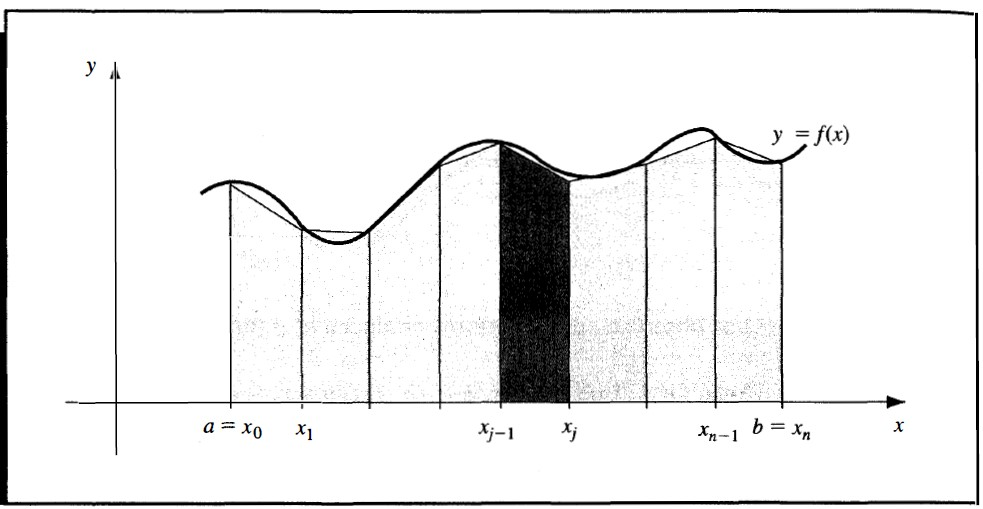
\includegraphics[scale=0.5]{Imagen12}
\end{frame}
%==========================================================================
\begin{frame}{Integración Numérica X}
\begin{Teo}[Regla Compuesta de Simpson]
Suponga que $f\in C^4[a,b]$, $h=\dfrac{b-a}{n}$ y $x_j=a+jh$. Existe $\mu\in(a,b)$ tal que la regla compuesta del trapecio se puede escribir junto con el error:
$$\int_{a}^{b}f(x)dx=\dfrac{h}{3}\bigg[ 	f(a)+2\sum_{j=1}^{n/2-1}f(x_{2j})+4\sum_{j=1}^{n/2}f(x_{2j-1})+f(b)\bigg]-\dfrac{b-a}{80}h^4f^{(4)}(\mu).$$
\end{Teo}
\begin{figure}[H]
\centering
\begin{tabular}{|c|}
\hline
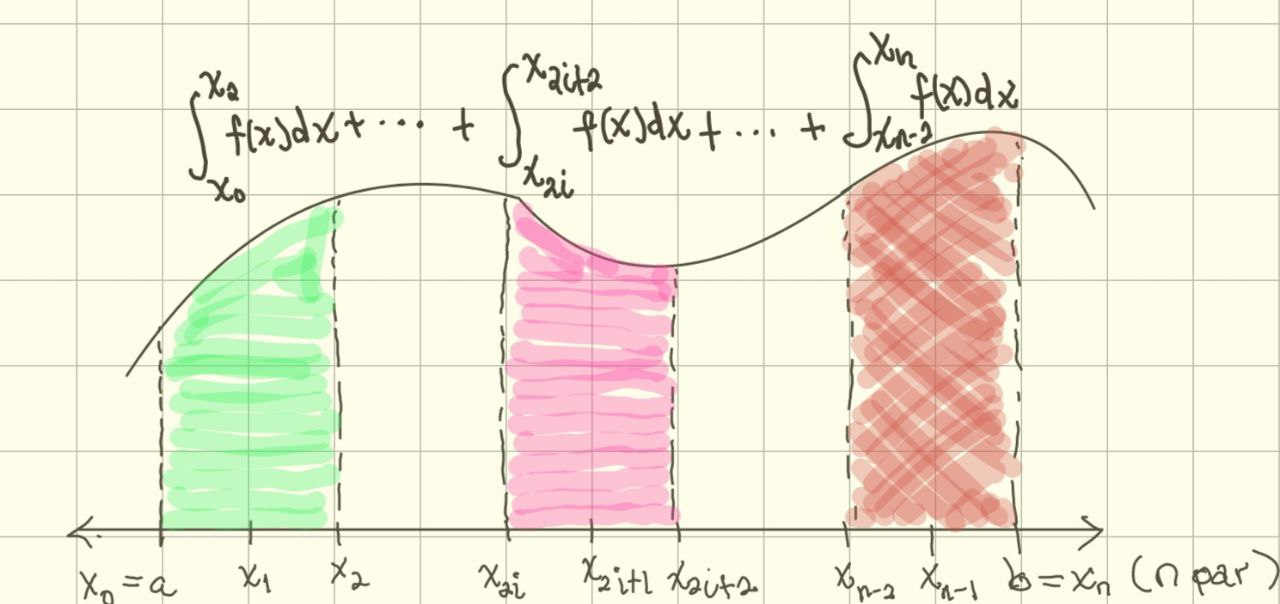
\includegraphics[scale=0.15]{Imagen11}\\
\hline
\end{tabular}
\end{figure}
\end{frame}
%==========================================================================
\begin{frame}{Integración Numérica XI}
\begin{Def}[Polinomios de Legendre]
Se define el conjunto de polinomios de Legendre $\{P_k(x)\}$, $k \in \{0,1,2,...\}$ a través de las siguientes propiedades:
\begin{itemize}
\item Para cada $k$, $P_k(x)$ es un polinomio de grado $k$.
\item $\displaystyle \int_{-1}^{1}P(x)P_k(x)dx=0 $ para todo polinomio $P(x)$ de grado menor que $k$. 
\end{itemize}
\end{Def}\pause
\textcolor{red}{Si el coeficiente principal del polinomio de Legendre es 1, entonces este es único; de lo contratrio podrían variar por algún factor real. }
\begin{Def}[Polinomios de Legendre]
Los polinomios de Legendre se definen explícitamente como:
$$P_n(x)=\dfrac{1}{2^n}\sum_{k=0}^{n}\binom{n}{k}^2(x+1)^{n-k}(x-1)^k$$
\end{Def}
\end{frame}
%==========================================================================
\begin{frame}{Integración Numérica XII}
\begin{Def}[Fórmula de cuadratura Gaussiana]
Sean ${x_i}_{i=1}^{n}$ las raíces del polinomio de Legendre $P_n(x)$. Defina los $c_i$ de la siguiente forma:
$$c_i=\int_{-1}^{1}\prod _{j=1,j\neq i}^{n}\dfrac{x-x_j}{x_i-x_j}dx$$
La fórmula de cuadratura Gaussiana es:
$$\int_{-1}^{1}f(x)\approx\sum_{i=1}^{n}c_if(x_i).$$
Si $f(x)$ es cualquier polinomio de grado menor que $2n$, entonces la aproximación es exacta y por lo tanto el grado de precisión es de $2n-1$.
\end{Def}
\end{frame}
